\section{Can Children's Verbal Use Explain Pronoun Case Errors? }
\subsection{Nominative case licensing}
The syntactic explanations focus on the non-nominative subject errors, where the accusative pronoun and the genitive pronoun are used as the subject (e.g. *\textit{me/my} eat it). In the syntactic theory, all structural cases are licensed by the head of a projection \citep[see][]{chomsky2000minimalist}. The nominative case is licensed by the \textsc{+finite} feature at the InflP level \citep[e.g.][]{haider1985unified, alec1991case} and the genitive case is licensed by the head of the DP \citep[e.g.][]{ritter1991two}. There are still debates about how the accusative case is assigned but it is agreed that it is assigned at the VP level or PP level. Other than structural cases, there is a default case in English, which is a case that doesn't denote grammatical relations or theta roles, but a filler when the case system failed to be checked. In English, the default case is the accusative case \citep{schutze1997, schutze2001}. For example, in sentences like `\textit{Who wants a cookie? - \textbf{Me}}', or `\textit{\textbf{Me} too}.' the accusative cased pronoun `me' is used as the default. Since the nominative case is licensed by the \textsc{+finite}, when a non-finite verb is used in a sentence, the system fails to check the nominative case. Thus the subject of the sentence will get the default case, which is the accusative case in English. For example, in the sentence `I went to school yesterday', the verb `went' is finite, thus the nominative case can be checked, resulting in `I' being the subject of the sentence. However, if the verb is non-finite in the sentence (e.g. the uninfected form of \textit{'went'}, '\textit{go}'), the nominative case won't get checked, resulting in the default accusative case used as the subject. Thus the sentence would be *`\textit{me} \textit{go} to school yesterday.' Young children often experience an Optional Infinitive stage \citep{wexler1994, wexler1998, wexler2000}, during which children would use non-finite verbs in their utterances. Although the theory doesn't explain why would children knowingly use the non-finite verb by omitting some verbal inflections, when the children use the non-finite verb, they would end up using the default accusative case as the subject, which leads to the non-nominative subject errors \citep{schutze1996subject, schutze1997}.  

The \textsc{+finite} feature in English can be realized in tense(\textsc{tns}), and/or person and number agreement (\textsc{arg}, e.g. third person singular agreement). The nominative case can be checked when any of the \textsc{+finite} features is present on the verbs, resulting in different configurations of the subject case and finite/non-finite verbs. Table \ref{tab: pattern} shows the predicted possible configuration of subject case and finiteness. 

\FloatBarrier
\begin{table}[!h]
    \centering
    \caption{The Configurations of finitenss with subject case (adapt from \cite{pine2005testing})}
    \begin{tabular}{llll}
    \toprule
        \textsc{Finiteness} & Case  & Examples  \\
    \hline
    Predicted to occur & & \\
         \textsc{+ arg, + tns} & \textsc{+ nom} & I am going. He goes. She's gone. She went.\\
         \textsc{- arg, - tns} & \textsc{- nom} & Me going. Him go. Her gone. Her went. \\
         (Omission of the inflections)\\
         \textsc{- arg, - tns} & \textsc{+nom} & I going. He goes. She's gone. \\
       \hline
       Predicted not to occur & & \\
       \textsc{+ arg, + tns} &  \textsc{-nom} & *\textit{Me am going. *Him goes. *Her's gone.} \\
        \bottomrule
    \end{tabular}
    \label{tab: pattern}
\end{table}
\FloatBarrier
In sum, the syntactic theory claims that the non-nominative subject error stems from the use of the non-finite verb. It predicts that when the verb is finite, the subject is almost never a non-nominative cased pronoun. 

\subsection{Testing the prediction}
The prediction was first tested on three children's data in CHILDES: Nina (1;11 - 2;5), Peter (1;11 - 2;5) and Sarah (2;8 - 3;1) \citep{schutze1996subject,schutze1997}. Only the pronoun subjects occurring with the unambiguous finite verbs and the unambiguous non-finite verbs were counted. The unambiguous finite verbs include auxiliaries, modals, copulas, past tense verbs, dummy \textit{do} and main verbs with \textit{-s}; and the unambiguous non-finite verbs include null auxiliary, null copula, main verbs and auxiliaries without \textit{-s}. Therefore, utterances like \textit{I go} or \textit{me go} are ignored. 
The tokens of nominative pronouns and non-nominative pronouns with finite verbs and non-finite verbs were tabulated and reproduced in Table \ref{table:schutzetotal} and Table \ref{tab:ATOMSchutze}. 
\FloatBarrier
\begin{table}[!h]
\centering
\caption{Total subject and verb form count for Nina, Peter, Sarah}
\label{table:schutzetotal}
\begin{tabular}{llll}
\toprule
 & \multicolumn{2}{l}{Verb Form} &\\ \cline{2-3} 
Subject & Finite & Non-Finite &\\ \hline
Nominative & 726  & 261  & 987 \\
Non-Nominative & 33  & 171  & 204 \\
\hline
& 759  & 432 & 1191  \\
\hline
 \multicolumn{4}{l}{Non-nominative finite rate = $\frac{33}{759}$ = 4.34\%} \\
\multicolumn{4}{l}{Finite non-nominative rate = $\frac{33}{204}$ = 16.18\%} \\
\bottomrule
\end{tabular}
\end{table}
\FloatBarrier

1191 subject pronouns were found that precede an unambiguous finite or non-finite verb in the corpus data of Nina, Peter and Sarah. Children generally use the subject correctly as 82.87\% of the subjects are nominative case. Children also use many non-finite verbs at this age, as only 63.73\% of the subjects precede a finite verb, fitting the description of the Optional Infinitival stage. Moreover, children have a strong tendency to use the nominative subjects with a finite verb. Of 759 pronoun subjects that precede a finite verb, only 33 of them are non-nominative pronouns, with an average non-nominative finite rate of 4.34\%. For different children and different pronouns, the non-nominative finite rate varies. For first person singular (1sg) pronoun, the rate is as low as 1.48\% for Peter and 3.08\% for Nina. For third person singular (3sg) pronouns, it was 7.09\% for Nina and 15.38\% for Sarah. The finite verbs following the non-nominative subjects are mostly past-tense verbs and modals, which only have \textsc{+tns} feature but not \textsc{+arg}. Therefore, \cite{schutze1997} concluded that `non-nominative subjects essentially never co-occur with agreeing verb forms'. In addition, \cite{schutze2001} further suggested that the non-nominative finite rate is so low that they can be regarded as noise in the data. 

However, the low non-nominative finite rate doesn't necessarily mean that non-nominative subjects almost never appear with a finite verb. First, there were too few data to confirm this finding: only three children's data were tested. Second, since children generally don't use that many non-nominative pronouns as the subject, there should be few non-nominative subjects that precede a finite verb. In addition, the non-nominative finite rate only calculates the percentage of non-nominative subjects of all the subjects precede a finite verb, which is not a fair representation of how often a non-nominative subject and a finite verb occur together. The percentage of the finite verbs of all verbs that follow a non-nominative pronoun should also be considered. Among 204 verbs that follow a non-nominative subject, 16.17\% of them are finite, which is not a low rate and shouldn't be counted as noise. The testing results in \cite{schutze1996subject} and \cite{schutze1997} only showed that when the non-nominative pronouns are used as subjects, the majority of them precede a non-finite verb, but didn't indicate that it's rare for them to precede a finite verb. 


\FloatBarrier
\begin{table}[!h]
    \caption{Reproducing \cite{schutze1997}'s data on Nina, Peter and Sarah}
    \label{tab:ATOMSchutze}
   \begin{minipage}[t]{0.5\textwidth}
    \centering
    \subcaption{Nina 1sg Finiteness VS Case}
    \small
    \begin{tabular}{@{}lll@{}}
        \toprule
         & \multicolumn{2}{c}{Verb form}\\
         \cline{2-3}
        Subject & Finite & Non-finite \\
        \midrule
        I & 189 & 63  \\
        me + my  & 6 & 18 \\
        \hline
         \multicolumn{3}{l}{Non-nominative finite rate = 3.08\%} \\
         \multicolumn{3}{l}{Finite non-nominative rate = 25\%}\\
        \bottomrule
    \end{tabular}
\end{minipage}
\vspace{1ex}
\begin{minipage}[t]{0.5\textwidth}
    \centering
    \subcaption{Nina 3sg Finiteness VS Case}
    \small
    \begin{tabular}{@{}lll@{}}
        \toprule
         & \multicolumn{2}{c}{Verb form}\\
         \cline{2-3}
        Subject & Finite & Non-Finite \\
        \midrule
        he + she & 249 & 149 \\
        him + her & 19 & 135 \\
        \hline
         \multicolumn{3}{l}{Non-nominative finite rate = 7.09\%} \\\multicolumn{3}{l}{Finite non-nominative rate = 12.33\%}\\
    \bottomrule
    \end{tabular}
    \end{minipage}
\vspace{1ex}
    %\caption{Nina Distribution by Verb Type}
    \begin{minipage}[t]{0.5\textwidth}
    \centering
    \subcaption{Nina 1sg Distribution by Verb Type}
    \small
    \begin{tabular}{lllll}
    \toprule
 &  & \multicolumn{3}{l}{Subject form} \\ \cline{3-5} 
Finiteness & Verb form & I & me & my \\ \hline
\multirow{2}{*}{\textsc{+arg}} & Auxiliary & 11 & 0 & 0 \\
 & Copula & 4 & 0 & 0 \\ \hline
\multirow{3}{*}{\textsc{+tns}} & Modal & 72 & 0 & 0 \\
 & Past Tense & 47 & 1 & 5 \\
 & Dummy \textit{do} & 55 & 0 & 0 \\ \hline
\multirow{2}{*}{\textsc{-finite}} & Null aux & 52 & 2 & 10 \\
 & Null cop & 11 & 2 & 4\\
\bottomrule
\end{tabular}
\end{minipage}
\vspace{1ex}
\begin{minipage}[t]{0.5\textwidth}
    \centering
    \subcaption{Nina 3sg Distribution by Verb Type}
    \small
\begin{tabular}{llllll}
\toprule
 &  & \multicolumn{4}{l}{Subject form} \\ \cline{3-6} 
Finiteness & Verb form & he & him & she & her \\ \hline
\multirow{3}{*}{\textsc{+arg}} & Main verb + \textit{`-s'} & 6 & 0 & 1 & 0 \\
 & Auxilliary + \textit{`-s'} & 113 & 0 & 3 & 3 \\
 & Copula + \textit{`-s'} & 88 & 3 & 2 & 4 \\ \hline
\multirow{2}{*}{\textsc{+tns}} & Modal & 13 & 1 & 1 & 2 \\
 & Past Tense & 20 & 0 & 2 & 6 \\ \hline
\multirow{4}{*}{\textsc{-finite}} & Main verb - \textit{`-s'} & 91 & 8 & 5 & 60 \\
 & Auxiliary - \textit{`-s'} & 19 & 0 & 1 & 14 \\
 & Null auxiliary & 24 & 1 & 0 & 27 \\
 & Null copula & 9 & 0 & 0 & 25\\
 \bottomrule
\end{tabular}
\end{minipage}
\vspace{1ex}
   \begin{minipage}[t]{0.5\textwidth}
    \centering
    \subcaption{Peter 1sg Finiteness VS Case}
    \small
    \begin{tabular}{@{}lll@{}}
        \toprule
         & \multicolumn{2}{c}{Verb form}\\
         \cline{2-3}
        Subject & Finite & Non-Finite \\
        \midrule
        I & 266 & 27 \\
        me + my  & 4 & 8\\
        \hline
         \multicolumn{3}{l}{Non-nominative finite rate = 1.48\%} \\
         \multicolumn{3}{l}{Finite non-nominative rate = 33.33\%}\\
        \bottomrule
    \end{tabular}
\end{minipage}
\vspace{1ex}
   \begin{minipage}[t]{0.5\textwidth}
    \centering
    \subcaption{Peter 1sg Distribution by Verb Type}
    \small
    \begin{tabular}{lllll}
    \toprule
 &  & \multicolumn{3}{l}{Subject form} \\ \cline{3-5} 
Finiteness & Verb form & I & me & my \\ \hline
\multirow{2}{*}{\textsc{+arg}} & Auxiliary & 126 & 0 & 0 \\
 & Copula & 10 & 0 & 0 \\ \hline
\multirow{3}{*}{\textsc{+tns}} & Modal & 54 & 0 & 0 \\
 & Past Tense & 74 & 3 & 1 \\
 & Dummy \textit{do} & 2 & 0 & 0 \\ \hline
\multirow{2}{*}{\textsc{-finite}} & Null aux & 27 & 4 & 2 \\
 & Null cop & 0 & 1 & 1\\
\bottomrule
\end{tabular}
\end{minipage}
\textbf{\linebreak}
\begin{minipage}[t]{0.5\textwidth}
    \centering
    \subcaption{Sarah 3sg Finiteness VS Case}
    \small
    \begin{tabular}{@{}lll@{}}
        \toprule
         & \multicolumn{2}{c}{Verb form}\\
         \cline{2-3}
        Subject & Finite & Non-Finite \\
        \midrule
        she & 22  & 22  \\
        her  & 4  & 10\\
        \hline
 \multicolumn{3}{l}{Non-nominative finite rate = 15.38\%} \\
\multicolumn{3}{l}{Finite non-nominative rate = 28.58\%}\\
        \bottomrule
    \end{tabular}
    \end{minipage}
\begin{minipage}[t]{0.5\textwidth}
    \centering
    \subcaption{Sarah 3sg Distribution by Verb Type}
    \small
 \begin{tabular}{llll}
\toprule
 &  & \multicolumn{2}{l}{Subject form} \\ \cline{3-4} 
Finiteness & Verb form & she & her \\ \hline
\multirow{3}{*}{\textsc{+arg}} & Main verb + \textit{`-s'} & 3 & 0 \\
 & Auxilliary + \textit{`-s'} & 6 & 0 \\
 & Copula + + \textit{`-s'} & 2 & 0 \\ \hline
\multirow{2}{*}{\textsc{+tns}} & Modal & 3 & 0 \\
 & Past Tense & 8 & 4 \\ \hline
\multirow{4}{*}{-finite} & Main verb - \textit{`-s'} & 9 & 7 \\
 & Auxiliary - \textit{`-s'} & 1 & 0 \\
 & Null auxiliary & 8 & 3 \\
 & Null copula & 4 & 0\\
 \bottomrule
\end{tabular}
\end{minipage}
\end{table}
\FloatBarrier

\cite{pine2005testing} proposed a straightforward way to test if the non-nominative subject almost never precedes a finite verb: by setting an upper limit as 10\%\footnote{They didn't explain the motivation to set the upper limite as 10\%.}, if the non-nominative finite rate is significantly larger than\footnote{A binomial test was used to compare the observed non-nominative rate and 10\%.} 10\%, then it is too frequent to be considered as noise. In their testing, they used a different criterion to select verb forms. Instead of using unambiguous finite and non-finite verbs, they used agreeing verbs and non-agreeing verbs. All the \textsc{+arg} verbs are considered as agreeing verbs, and the rest of the verbs are non-agreeing verbs, including \textsc{+tns} verbs, unambiguous non-finite verbs and ambiguous verbs. They first retested Nina's, Peter's and Sarah's data on 1sg pronoun and 3sg pronoun. Since there were no agreeing verbs that precede \textit{me} and \textit{my} in Nina's and Peter's data, they focused on the non-nominative rate of 3sg pronoun in Sarah's and Nina's data. Sarah didn't use any \textit{him} or \textit{her} that precede an agreeing verb either. For Nina, 4.48\% of the 3sg subjects that precede an agreeing verb are non-nominative pronouns, which is significantly smaller than 10\%. However, the masculine and feminine pronouns behave differently. The non-nominative pronoun \textit{her} takes 53.85\% of the 3sg feminine subjects with a finite verb, which is significantly greater than 10\%. The re-test result for Nina's 3sg subjects is reproduced in Table \ref{table:nina}.
\FloatBarrier
\begin{table}[!h]
\centering
\caption{Distribution of Nina's 3sg pronoun subject's case and agreeing verbs from in \cite{pine2005testing}}
\label{table:nina}
\begin{tabular}{lll}
\toprule
 & \multicolumn{2}{l}{Verb Form} \\ \cline{2-3} 
Subject & Agreeing & \begin{tabular}[c]{@{}l@{}}Non-\\ Agreeing\end{tabular} \\ \hline
He + She & 213 & 185 \\
Him/His + Her & 10 & 144 \\ \hline
\multicolumn{3}{l}{Non-nominative finite rate = $\frac{10}{213+10}$ = 4.48\%} \\ \hline
She & 6 & 9 \\
Her & 7 & 134 \\ \hline
\multicolumn{3}{l}{Non-nominative finite rate = $\frac{7}{6+7}$ = 53.85\%*}\\
\bottomrule
\end{tabular}
\end{table}

\FloatBarrier

In addition, they did the same test on four more children: Anne, Becky and Gail, from the Manchester corpus \citep{theakston2001} and Abe from  \cite{kuczaj1977acquisition}, who produced enough non-nominative 3sg subjects with agreeing verbs that can be properly tested. The average non-nominative finite rate for 3sg pronoun is 7.08\%, which is not significantly greater than 10\%. However, the rate for 3sg feminine pronoun is 43.01\%, which is significantly greater than 10\%.  The results are reproduced in Table \ref{tab:fourtotal}. 
\FloatBarrier
\begin{table}[!h]
\centering
\caption{Distribution of 3sg pronoun subject's case and agreeing verb forms for Anne, Becky, Gail and Abe}
\label{tab:fourtotal}
\begin{tabular}{lll}
\toprule
 & \multicolumn{2}{l}{Verb Form} \\ \cline{2-3} 
Subject & Agreeing & \begin{tabular}[c]{@{}l@{}}Non-\\ Agreeing\end{tabular} \\ \hline
He + She & 629 & 305 \\
Him/His + Her & 48 & 59 \\ \hline
\multicolumn{3}{l}{Non-nominative finite rate = $\frac{48}{629+48}$ = 7.08\%} \\ \hline
She & 53 & 41 \\
Her & 40 & 47 \\ \hline
\multicolumn{3}{l}{Non-nominative finite rate = $\frac{40}{53+40}$ = 43.0\%*}\\
\bottomrule
\end{tabular}
\end{table}
\FloatBarrier
This pattern is also true for each individual child. All four children's total 3sg non-nominative finite rate is significantly less than or no different from 10\%, but 3sg feminine non-nominative subject `her' consistently precedes a finite verb over 10\% of the time. The distribution of subject case and agreeing verbs for each child is reproduced in Table \ref{tab: Pine}.
\FloatBarrier
\begin{table}[!h]
\centering
\caption{Each child's distribution of 3sg pronoun subject's case and agreeing verb forms from \cite{pine2005testing}}
\label{tab: Pine}
\begin{tabular}{llll|lll}
\toprule
 &  & Agreeing & \begin{tabular}[c]{@{}l@{}}Non-\\ Agreeing\end{tabular} &  & Agreeing & \begin{tabular}[c]{@{}l@{}}Non-\\ Agreeing\end{tabular} \\ \hline
\multirow{3}{*}{Anne} & He+She & 131 & 73 & She & 8 & 11 \\
 & Him/His + Her & 5 & 6 & Her & 4 & 3 \\ \cline{2-7} 
 & \multicolumn{3}{l|}{Non-nominative finite rate = 3.4\%} & \multicolumn{3}{l}{Non-nominative finite rate = 33.3\%*} \\ \hline
\multirow{3}{*}{Becky} & He+She & 239 & 80 & She & 26 & 22 \\
 & Him/His + Her & 16 & 2 & Her & 13 & 0 \\ \cline{2-7} 
 & \multicolumn{3}{l|}{Non-nominative finite rate =  6.3\%} & \multicolumn{3}{l}{Non-nominative finite rate = 33.3\%*} \\ \hline
\multirow{3}{*}{Gail} & He+She & 146 & 48 & She & 14 & 3 \\
 & Him/His + Her & 13 & 16 & Her & 9 & 10 \\ \cline{2-7} 
 & \multicolumn{3}{l|}{Non-nominative finite rate =  8.2\%} & \multicolumn{3}{l}{Non-nominative finite rate = 39.1\%*} \\ \hline
\multirow{3}{*}{Abe} & He+She & 113 & 104 & She & 5 & 5 \\
 & Him/His + Her & 14 & 35 & Her & 14 & 34 \\ \cline{2-7} 
 & \multicolumn{3}{l|}{Non-nominative finite rate = 11.0\%} & \multicolumn{3}{l}{Non-nominative finite rate = 73.7\%*}\\
 \bottomrule
\end{tabular}
\end{table}
\FloatBarrier
Thus, \cite{pine2005testing} concluded that it is not true that the non-nominative subjects almost never precede a finite verb. For 3sg feminine pronoun, the non-nominative form \textit{her} appears with a finite verb quite frequently and of all the 3sg feminine subjects that precede a finite verb 43\% of them are \textit{her}. The data doesn't support the prediction of the syntactic explanation that the non-nominative subject almost never occurs with a finite verb. In addition, children generally don't use many non-nominative pronouns as the subject, and there are even less of them that precede a finite verb, which makes the syntactic prediction particularly difficult to test. 

\subsection{Re-testing the prediction}
The syntactic explanation claims that the use of the non-finite verb is the reason for the non-nominative subject. It predicts that there should be no non-nominative subjects preceding a finite verb; and if there are any in the children's data, those are just noise. In different children's corpus data, the average non-nominative finite rate for the 1sg and the 3sg pronouns is significantly lower than 10\%, which some argue that could be treated as noise. However, the 3sg feminine pronoun's non-nominative finite rate is significantly larger than 10\%, which contradicts the prediction. This section reviews the existing testing methods and argues that the non-nominative finite rate should not be judged by its surface value. The low rate doesn't necessarily mean that the non-nominative subjects rarely precede a finite verb.

In \cite{schutze1996subject} and \cite{pine2005testing}, the non-nominative finite rate is calculated as the number of non-nominative subjects preceding a finite verb over the total subject pronouns that precede a finite verb, or cell `c' over the sum of cell `a' and `c' in the 2x2 contingency table in Table \ref{tab:2x2}. 

\begin{equation}
\label{equ:1}
\centering
     \text{non-nominative finite rate} = \displaystyle\frac{\text{non-nominative finite subjects }}{\text{total finite pronoun subjects}} = \displaystyle\frac{\text{c}}{\text{a+c}}
\end{equation}

\FloatBarrier
\begin{table}[!h]
\centering
\caption{2x2 Contingency Table of subject case and verb form}
\label{tab:2x2}
\begin{tabular}{lll}
\toprule
 & \multicolumn{2}{l}{Verb Form} \\ \cline{2-3} 
 & Finite & Non-finite \\
Nominative & a & b \\
Non-nominative & c & d\\
\bottomrule
\end{tabular}
\end{table}
\FloatBarrier

The non-nominative finite rate calculated in Equation \ref{equ:1}  actually is the conditional probability of a  non-nominative subject given a finite verb: 
\begin{align*}
\label{equ:44}
\centering
\text{non-nominative finite rate} & = \text{P(Non-nominative|Finite)}\\
&= \displaystyle\frac{\text{P(Non-nominative $\cap$ Finite)}}{\text{P(Finite)}}\\
& = \displaystyle\frac{\displaystyle\frac{\text{c}}{\text{a+b+c+d}}}{\displaystyle\frac{\text{a+c}}{\text{a+b+c+d}}} = \displaystyle\frac{\text{c}}{\text{a+c}}
\end{align*}
Therefore, the surface value of the rate doesn't truly reflect if a non-nominative subject never occurs with a finite verb. In order to decide whether the presence of a finite verb blocks the use of a non-nominative subject, the rate needs to be compared to the probability of non-nominative subject P(Non-nominative). If P(Nominative) and P(Finite) are independent events, meaning that the presence of finite verb does not affect the use of non-nominative subjects, the conditional probability P(Non-nominative|Finite) equals P(Non-nominative): 
\begin{align*}
   \text{P(Non-nominative|Finite)} &= 
   \displaystyle\frac{\text{P(Non-nominative $\cap$ Finite)}}{\text{P(Finite)}}\\
   &= \displaystyle\frac{\text{P(Non-nominative) $\times$ P(Finite)}}{\text{P(Finite)}}\\
   &= \text{P(Non-nominative)}\\
   &= \displaystyle\frac{\text{c+d}}{\text{a+b+c+d}}
\end{align*}
If P(Non-nominative|Finite)is significantly smaller than P(Non-nominative), it means that P(Non-nominative) and P(Finite) are not independent, indicating that the presence of the finite verb prevents the non-nominative subjects. For example, assume that P(Non-nominative) is only 5\%, if  P(Non-nominative|Finite) is 1\%, which is even smaller than 5\%, then it is even more unlikely to see a non-nominative subject when there is a finite verb. However, if P(Non-nominative|Finite) is 8\%, it suggests that the presence of the finite verb actually increases the probability of a non-nominative subject, although 8\% is a relatively low rate.  

Therefore, the P(Non-nominative|Finite) ($\displaystyle\frac{\text{c}}{\text{a+c}}$) should be compared to P(Non-nominative) ($\displaystyle\frac{\text{c+d}}{\text{a+b+c+d}}$), and if it is significantly smaller than P(Non-nominative), it can be concluded that the non-nominative subject almost never appears before a finite verb. The log-likelihood ratio test (the \textit{G}-test) was used to compare P(Non-nominative|Finite) and P(Non-nominative). The G-statistic can be calculated as the natural log of the observed number (\textit{O}) divided by the expected number (\textit{E}) and multiply by 2. The formula for G is:
\begin{equation}
    \centering
    G = 2 \times \displaystyle\sum_{i = 1}^{n}(O_i \times ln(\displaystyle\frac{\text{$O_i$}}{\text{$E_i$}}))
\end{equation}

The observed numbers are the number of nominative and non-nominative subjects preceding a finite verb, which are cell `a' and cell `c' in the 2x2 contingency table, as shown in Table \ref{tab:tada}. The expected numbers are the pronoun subjects preceding a finite verb assuming that P(Non-nominative) and P(Finite) are independent. The expected number of nominative finite subjects ($E_{Nominative}$) and expected non-nominative finite subjects ($E_{Non-nominative}$) is calculated as the total numbers of subjects precede a finite verb times P(Nominative|Finite) and P(Non-nominative|Finite):
\begin{align*}
    E_{Nominative} & = \text{(a+c)} \times \text{P(Nominative|Finite)} \\
    & = \text{(a+c)} \times \text{P(Nominative)} \\
    & = \text{(a+c)} \times \displaystyle\frac{\text{a+b}}{\text{a+b+c+d}}\\
    & = \displaystyle\frac{\text{(a+c)(a+b)}}{\text{a+b+c+d}}
\end{align*}
\begin{align*}
    E_{Non-nominative} & = \text{(a+c)} \times \text{P(Non-nominative|Finite)} \\
    & = \text{(a+c)} \times \text{P(Non-nominative)} \\
    & = \text{(a+c)} \times \displaystyle\frac{\text{c+d}}{\text{a+b+c+d}} \\
     & = \displaystyle\frac{\text{(a+c)(c+d)}}{\text{a+b+c+d}}
\end{align*}
\FloatBarrier
\begin{table}[!h]
\centering
\caption{Observed and Expected numbers and P(Non-nominative) and \text{r\%} represented by cell numbers in 2x2 contingency table}
\label{tab:tada}
\begin{tabular}{llll}
\toprule
 & \begin{tabular}[c]{@{}l@{}}Total Pronoun  \\
Subjects\end{tabular} &\begin{tabular}[c]{@{}l@{}}Observed \\
 Agreeing Subjects\end{tabular} & \begin{tabular}[c]{@{}l@{}}Expected \\ Agreeing Subjects\end{tabular} \\ 
 \hline 
Nominative & a+b & a & \displaystyle\frac{\text{(a+c)(a+b)}}{\text{a+b+c+d}} \\[1.5ex]
\hline 
Non-nominative & c+d & c & \displaystyle\frac{\text{(a+c)(c+d)}}{\text{a+b+c+d}} \\ [1.5ex]
\hline
\multicolumn{4}{l}{P(Non-nominative) = \displaystyle\frac{\text{c+d}}{\text{a+b+c+d}}, \text{P(Non-nominative|Finite)} = \displaystyle\frac{\text{c}}{\text{a+c}}}\\
\bottomrule
\end{tabular}
\end{table}
\FloatBarrier


The data reported in \cite{schutze1997} and \cite{pine2005testing} were used to calculated the G-statistics of P(Non-nominative) and P(Non-nominative|Finite) in 1sg pronouns and 3sg pronouns. Following \cite{pine2005testing}, finite verbs were counted as agreeing verbs. The test result of 1sg pronouns is shown in Table \ref{Tab:gtest1}\footnote{The counts are different from Table \ref{tab:ATOMSchutze} because different verb selection criteria were applied. In Table \ref{tab:ATOMSchutze}, finite forms only included the unambiguous \textsc{+tns} and/or \textsc{+arg} verbs, and non-finite forms only included the unambiguous non-finite verbs. In Table \ref{Tab:gtest1}, only agreeing verbs were counted as finite verbs.}. Both Nina's P(Non-nominative|Finite) (3.07\%) and Peter's P(Non-nominative|Finite) (1.48\%) are significantly smaller than their P(Non-nominative), suggesting that the non-nominative first person pronoun (\textit{me} and \textit{my}) rarely precedes a non-finite verb. 

\FloatBarrier
\begin{table}[!h]
\centering
\caption{G-test for 1sg pronoun for Nina and Peter (data reproduced from \cite{schutze1997})}
\label{Tab:gtest1}
\begin{tabular}{lllll}
\toprule
 & & \begin{tabular}[c]{@{}l@{}}Total Pronoun \\ Subjects\end{tabular} & \begin{tabular}[c]{@{}l@{}}Observed \\ Agreeing Subjects\end{tabular} & \begin{tabular}[c]{@{}l@{}}Expected \\ Agreeing Subjects\end{tabular} \\ \hline
\multirow{3}{*}{Nina} & I & 903 & 189 & 169.31 \\ \cline{2-5} 
 & me + my & 137 & 6 & 25.68 \\ \cline{2-5} 
 & & \multicolumn{3}{l}{P(Non-nominative)\% = 13.17\%, P(Non-nominative|Finite)\% = 3.07\%}\\
 & &\multicolumn{3}{l}{\textbf{G = 24.13***}, p <0.001} \\ \hline
\multirow{3}{*}{Peter} & I & 700 & 266 & 243.56 \\ 
\cline{2-5}
 & me + my & 76 & 4 & 26.44 \\ \cline{2-5} 
 & & \multicolumn{3}{l}{P(Non-nominative)\% = 9.79\%, P(Non-nominative|Finite)\% =1.48\%}\\
 &&\multicolumn{3}{l}{\textbf{G = 31.78***}, p<0.001} \\
 \bottomrule
\end{tabular}
\end{table}
\FloatBarrier

In addition, more children's 1sg data were added to test for the G-statistics. The selection criteria include: (1) the children have to produce enough non-nominative subject errors, which means P(Non-nominative) $\geq$ 2\%; (2) the children have to produce more than 2 non-nominative subjects that precede a finite verb, which means cell `c' $\geq$ 2. Only seven more children fit the selection criteria: Ruth, Nicole, Warren and Anne from the Manchester corpus \citep{theakston2001}, Laura from \cite{braunwald1971mother}, Eve from Brown corpus \citep{brown1973first} and Naomi from \cite{sachs1983talking}. The G-test results for the seven more children are shown in Table \ref{tab:7more}. Only three children's P(Non-nominative|Finite) is significantly smaller than P(Non-nominative): Ruth's 48.68\% < 60.04\%; Warren's 2.62\% < 6.56\% and Anne's 1.42\% < 3.19\%. For the other four children, their 1sg pronoun's  P(Non-nominative|Finite) is not significantly smaller than P(Non-nominative), indicating that the presence of a finite verb doesn't prevent \textit{me} and \textit{my} being used as the subject.  

The results of 3sg masculine and feminine pronouns are shown in Tables \ref{tab:himhigtest} and \ref{tab:hershegtest}. Although 3sg masculine pronoun's P(Non-nominative|Finite) is extremely low for all four children, ranging from 2.94\% to 0.75\%, none of the P(Non-nominative|Finite) is significantly smaller than P(Non-nominative), indicating that the finite verb doesn't prevent the non-nominative pronouns \textit{him} and \textit{his} from preceding an agreeing verb. The 3sg feminine pronoun's P(Non-nominative) are all relatively high for all five children, ranging from 33.33\% to 73.68\%. For Anne and Becky, their P(Non-nominative|Finite) (33.33\% for both) are even larger than their P(Non-nominative) (26.92\% and 21.31\% respectively). However, none of the P(Non-nominative) is significantly different from P(Non-nominative|Finite), except for Nina. Nina mostly used \textit{her} as a subject; she has the highest P(Non-nominative), which is 90.38\%, but her P(Non-nominative|Finite) is 62.5\%, which is significantly smaller than P(Non-nominative). The G-test results demonstrate that it is not rare for \textit{her} as a subject to precede a finite verb.

In addition, all children's 1sg and 3sg pronouns' P(Non-nominative) and P(Non-nominative|Finite) were combined for a meta-analysis. Table \ref{tab: Pnon} shows each child's P(Non-nominative) and P(Non-nomiantive|Finite)\footnote{For Nina and Anne, the non-nominative pronouns include the total counts of 1sg \textit{me/my}and 3sg pronouns \textit{him/his} and \textit{her}. For Becky and Gail, the non-nominative pronouns included the total counts of 3sg pronouns \textit{him/his} and \textit{her}.}. An exact sign test shows that the median difference in P(Non-nominative) and P(Non-nominative|Finite) is significant (p = 0.004), meaning that the presence of a finite verb decreases the possibility of a non-nominative pronoun being used as a subject by 2.81\%. 

\FloatBarrier
\begin{table}[h]
\centering
\caption{12 Children's P(Non-nominative) and P(Non-nomiantive|Finite)}
\label{tab: Pnon}
\begin{tabular}{l|cc}
\toprule
 & P(Non-nominative) & P(Non-nominative|Finite) \\
 \hline
Peter & 9.79\% & 1.48\% \\
Ruth & 60.04\% & 48.68\% \\
Nicole & 5.35\% & 3.68\% \\
Warren & 6.56\% & 2.62\% \\
Laura & 2.22\% & 2.06\% \\
Eve & 2.03\% & 1.95\% \\
Naomi & 2.10\% & 1.20\% \\
Abe & 82.76\% & 73.68\% \\
Nina & 18.19\% & 5.40\% \\
Anne & 3.5\% & 2.01\% \\
Becky & 5.34\% & 6.27\% \\
Gail & 13\% & 8.18\% \\
\hline
median & 5.96\% & 3.15\%\\
\bottomrule
\end{tabular}
\end{table}
\FloatBarrier
In addition, in order to test if the P(Non-nominative|Finite) is smaller than P(Non-nominative) for 1sg, 3sg masculine and 3sg feminine pronouns, the p-values of children's G-test were combined using Fisher's method. The formula is shown in Equation \ref{equ3}, where p_i is the p-value for each G-test, k is the number of tests being combined. $\chi^2$ has a chi-squared distribution with $2k$ degrees of freedom.
\begin{equation}
\label{equ3}
    \chi^2_{2k} \sim -2\displaystyle\sum^k_{i=1}ln(p_i)
\end{equation}
For 9 children with 1sg pronoun's data, the $\chi^2$ is 101.7. The critical value (p<0.05) of chi-square for df = 18 is 28.87, indicating that P(\textit{me+my }|Finite) is significantly smaller than P(\textit{me+my}). For 5 children with 3sg feminine pronoun's data, the $\chi^2$ is 28.12. The critical value (p<0.05) of chi-square for df = 10 is 18.31, suggesting that P(\textit{her }|Finite) is significantly smaller than P(\textit{her}). For 4 children with 3sg masculine pronoun's data, the $\chi^2$ is 11.52. The critical value (p<0.05) of chi-square for df = 8 is 15.51, showing that P(\textit{him+his }|Finite) is not significantly different from P(\textit{him+his}). 


In conclusion, the meta-analysis shows that P(Non-nominative|Finite) is generally significantly smaller than P(Non-nominative), suggesting that the finite verb could decrease the possibility of a non-nominative pronoun being used as the subject. However, there is great variance among different children and different pronouns. For 1sg pronoun, 4 out of 9 children's P(\textit{me+my}) is not significantly different from P(\textit{me+my}|Finite). For 3sg masculine pronoun, all 4 children's P(\textit{him+his}|Finite) is not different from P(\textit{him+his}). For 3sg feminine pronoun, 4 out of 5 children's P(\textit{her}) is not different from P(\textit{her}|Finite). 

\FloatBarrier
\begin{table}[!h]
\centering
\caption{G-test of 1sg pronoun for seven more children}
\label{tab:7more}
\begin{tabular}{lllll}
\toprule
 &  & \begin{tabular}[c]{@{}l@{}}Total Pronoun\\ Subjects\end{tabular} & \begin{tabular}[c]{@{}l@{}}Observed\\ Agreeing Subjects\end{tabular} & \begin{tabular}[c]{@{}l@{}}Expected\\ Agreeing Subjects\end{tabular} \\ \hline
\multirow{3}{*}{Ruth} & I & 591 & 78 & 60.74 \\ \cline{2-5} 
 & me + my & 888 & 74 & 91.26 \\ \cline{2-5} 
 &  & \multicolumn{3}{l}{P(Non-nominative) = 60.04\%, P(Non-nominative|Finite) = 48.68\%}\\
 & & \multicolumn{3}{l}{\textbf{G = 7.99**}, p \textless 0.01} \\ \hline
\multirow{3}{*}{Nicole} & I & 478 & 131 & 128.73 \\ \cline{2-5} 
 & me + my & 27 & 5 & 7.27 \\ \cline{2-5} 
 &  & \multicolumn{3}{l}{P(Non-nominative) = 5.35\%, P(Non-nominative|Finite) = 3.68\%} \\
 & & \multicolumn{3}{l}{G = 0.84, p = 0.36} \\ \hline
\multirow{3}{*}{Warren} & I & 1354 & 297 & 285.00 \\ \cline{2-5} 
 & me + my & 95 & 8 & 20.00 \\ \cline{2-5} 
 &  & \multicolumn{3}{l}{P(Non-nominative) = 6.56\%, P(Non-nominative|Finite) = 2.62\%}\\
 & & \multicolumn{3}{l}{\textbf{G = 9.83**}, p \textless 0.01} \\ \hline
\multirow{3}{*}{Anne} & I & 1000 & 346 & 339.79 \\ \cline{2-5} 
 & me + my & 33 & 5 & 11.21 \\ \cline{2-5} 
 &  & \multicolumn{3}{l}{P(Non-nominative) = 3.19\%, P(Non-nominative|Finite) = 1.42\%}\\
 & & \multicolumn{3}{l}{\textbf{G = 4.46*}, p \textless 0.05} \\ \hline
\multirow{3}{*}{Laura} & I & 3210 & 1188 & 1186.03 \\ \cline{2-5} 
 & me + my & 73 & 25 & 26.97 \\ \cline{2-5} 
 &  & \multicolumn{3}{l}{P(Non-nominative) = 2.22\%, P(Non-nominative|Finite) = 2.06\%} \\
 & & \multicolumn{3}{l}{G = 0.15, p = 0.70} \\ \hline
\multirow{3}{*}{Eve} & I & 1256 & 251 & 250.81 \\ \cline{2-5} 
 & me + my & 26 & 5 & 5.19 \\ \cline{2-5} 
 &  & \multicolumn{3}{l}{P(Non-nominative) = 2.03\%, P(Non-nominative|Finite) = 1.95\%} \\
 & & \multicolumn{3}{l}{G = 0.01, p = 0.93} \\ \hline
\multirow{3}{*}{Naomi} & I & 1820 & 657 & 651.05 \\ \cline{2-5} 
 & me + my & 39 & 8 & 13.95 \\ \cline{2-5} 
 &  & \multicolumn{3}{l}{P(Non-nominative) = 2.10\%, P(Non-nominative|Finite) = 1.20\%} \\
 & & \multicolumn{3}{l}{G = 3.06, p =0.08}\\
 \bottomrule
\end{tabular}
\end{table}
\FloatBarrier


\FloatBarrier
\begin{table}[!h]
\centering
\caption{G-test for 3sg masculine pronoun for Nina, Anne, Becky and Gail (data reproduced from \cite{pine2005testing})}
\label{tab:himhigtest}

\begin{tabular}{lllll}
\toprule
 &  & \begin{tabular}[c]{@{}l@{}}Total Pronoun\\ Subjects\end{tabular} & \begin{tabular}[c]{@{}l@{}}Observed\\ Agreeing Subjects\end{tabular} & \begin{tabular}[c]{@{}l@{}}Expected\\ Agreeing Subjects\end{tabular} \\ \hline
\multirow{3}{*}{Nina} & he & 391 & 240 & 236.15 \\ \cline{2-5} 
 & him + his & 13 & 4 & 7.85 \\ \cline{2-5} 
 &  & \multicolumn{3}{l}{P(Non-nominative) = 3.22\%, P(Non-nominative|Finite) = 1.64\%}\\
 & & \multicolumn{3}{l}{G = 2.37, p = 0.12} \\ \hline
\multirow{3}{*}{Anne} & he & 195 & 133 & 131.31 \\ \cline{2-5} 
 & him + his & 4 & 1 & 2.69 \\ \cline{2-5} 
 &  & \multicolumn{3}{l}{P(Non-nominative) = 2.01\%, P(Non-nominative|Finite) = 0.75\%}\\
 & & \multicolumn{3}{l}{G = 1.43, p = 0.23} \\ \hline
\multirow{3}{*}{Becky} & he & 271 & 213 & 212.09 \\ \cline{2-5} 
 & him + his & 5 & 3 & 3.91 \\ \cline{2-5} 
 &  & \multicolumn{3}{l}{P(Non-nominative) = 1.81\%, P(Non-nominative|Finite) = 1.39\%}\\
 & & \multicolumn{3}{l}{G = 0.24, p = 0.63} \\ \hline
\multirow{3}{*}{Gail} & he & 177 & 132 & 128.73 \\ \cline{2-5} 
 & him + his & 10 & 4 & 7.27 \\ \cline{2-5} 
 &  & \multicolumn{3}{l}{P(Non-nominative) = 5.35\%, P(Non-nominative|Finite) = 2.94\%}\\
 & & \multicolumn{3}{l}{G = 1.85, p = 0.17}\\
 \bottomrule
\end{tabular}
\end{table}
\begin{table}[!h]
\centering
\caption{G-test for 3sg feminine pronoun for Nina, Anne, Becky and Gail (data reproduced from \cite{pine2005testing})}
\label{tab:hershegtest}
\begin{tabular}{lllll}
\toprule
 &  & \begin{tabular}[c]{@{}l@{}}Total Pronoun\\ Subjects\end{tabular} & \begin{tabular}[c]{@{}l@{}}Observed\\ Agreeing Subjects\end{tabular} & \begin{tabular}[c]{@{}l@{}}Expected\\ Agreeing Subjects\end{tabular} \\ \hline
\multirow{3}{*}{Nina} & she & 15 & 9 & 2.31 \\ \cline{2-5} 
 & her & 141 & 15 & 21.69 \\ \cline{2-5} 
 &  & \multicolumn{3}{l}{P(Non-nominative) = 90.38\%, P(Non-nominative|Finite) = 62.5\%}\\
 & & \multicolumn{3}{l}{G = \textbf{13.43***}, p \textless{}0.001} \\ \hline
\multirow{3}{*}{Anne} & she & 19 & 8 & 8.77 \\ \cline{2-5} 
 & her & 7 & 4 & 3.23 \\ \cline{2-5} 
 &  & \multicolumn{3}{l}{P(Non-nominative) = 26.92\%, P(Non-nominative|Finite) = 33.33\%}\\
 & & \multicolumn{3}{l}{G = 0.24, p = 0.62} \\ \hline
\multirow{3}{*}{Becky} & she & 48 & 26 & 30.69 \\ \cline{2-5} 
 & her & 13 & 13 & 8.31 \\ \cline{2-5} 
 &  & \multicolumn{3}{l}{P(Non-nominative) = 21.31\%, P(Non-nominative|Finite) = 33.33\%}\\
 & & \multicolumn{3}{l}{G = 3.01, p = 0.08} \\ \hline
\multirow{3}{*}{Gail} & she & 17 & 14 & 10.86 \\ \cline{2-5} 
 & her & 19 & 9 & 12.14 \\ \cline{2-5} 
 &  & \multicolumn{3}{l}{P(Non-nominative) = 52.78\%, P(Non-nominative|Finite) = 39.13\%}\\
 & & \multicolumn{3}{l}{G = 1.72, p = 0.19}\\
 \hline
\multirow{3}{*}{Abe} & she & 10 & 15 & 3.28 \\ \cline{2-5} 
 & her & 48 & 14 & 15.72 \\ \cline{2-5} 
 &  & \multicolumn{3}{l}{P(Non-nominative) = 82.76\%, P(Non-nominative|Finite) = 73.68\%}\\
 & & \multicolumn{3}{l}{G = 0.98, p = 0.32}
\\ \bottomrule
\end{tabular}
\end{table}
\FloatBarrier

\subsection{The correlation between verbal finiteness and nominative case correct rate}
\label{section:rispoli20051}

In addition to \cite{schutze1996subject}, \cite{schutze1997} and \cite{pine2005testing}'s attempts to test the syntactic prediction with children's longitudinal data, researchers also tried to verify the relationship between verbal finiteness and pronoun case errors by establishing significant correlations with children's cross-sectional data. \cite{rispoli2005} found a significant negative correlation between the verbal finiteness and pronoun case error rate, which supports the syntactic prediction. This section discusses his methods and replicates the tests on the cross-sectional data in CHILDES. 

\cite{rispoli2005} collected spontaneous speech data from 44 children ranging from the age of 2;0 to 4;0. Each child was recorded twice during their play session for one hour. Rispoli counted all types of the case errors of 3sg and 3pl pronouns (e.g. \textit{him} for \textit{he}, \textit{him} for \textit{his} and \textit{he} for \textit{him}). The error rate is calculated as the error count divided by the total attempts (combining both errors and successful attempts). He also counted all the sentences with a noun subject that precedes a finite verb. The percentage of such sentences is children's finiteness rate. The error rate for all types of case errors ranges from 0 to 0.70 (mean = 0.17 S.D. = 0.21). The range of error rate for  \textit{him}-for-\textit{he} error is 0 to 0.29 (mean = 0.05, S.D. = 0.08), for \textit{her}-for-\textit{she} error is 0 to 0.37 (mean = 0.07, S.D. = 0.11) and for \textit{them}-for-\textit{they} error is 0 to 0.16 (mean =  0.02, S.D = 0.04). The range of finiteness rate was 0.11 - 0.97 (M = 0.48, S.D = 0.24). The Pearson correlation shows that there is no correlation between case error rate and age and MLU. There is a significantly negative correlation between error rate and finiteness rate (r = -0.38*). He also found a negative correlation between error rate and SDpro (r = -0.44**), which is a measure of the dispersion of children's pronoun production created by Rispoli. The higher the SDpro, the more concentrated the children's pronoun production is in few pronouns. The detailed calculation of SDpro and the relationship between SDpro and pronoun case error will be discussed in \ref{section:rispoli20052}. The correlation table is reproduced in Table \ref{tab:corRis}. 
\FloatBarrier
\begin{table}[!h]
\centering
\caption{Correlation between age, MLU, Finiteness and SDpro in \cite{rispoli2005}}
\label{tab:corRis}
\begin{tabular}{llllll}
\toprule
N = 44 & 1& 2 & 3 & 4 & 5 \\
 \hline
1.Error Rate & 1&  0.14 & 0.05 & \textbf{-0.38*} & \textbf{-0.44*} \\
2. Age &  &1& \textbf{0.38*} & 0.29 & \textbf{-0.34*} \\
3. MLU &  &  & 1&\textbf{0.57**} & -0.30 \\
4. Finiteness &  &  &  &1& \textbf{-0.33*}\\
5. SDpro& & & & & 1\\
\bottomrule
\end{tabular}
\end{table}
\FloatBarrier
Rispoli further calculated the partial correlation between pronoun case error rate and the finiteness rate, controlling for SDpro. The correlation increased to -0.61, meaning that the correlation between Error Rate and Finiteness is not due to SDpro. Therefore, he concluded that the negative correlation between error rate and the finiteness supports the syntactic hypothesis that the knowledege of finitness is important for children to make fewer pronoun case errors.
\begin{equation}
       r_{14.5} &= \displaystyle\frac{r_{14}-r_{15}r_{45}}{\sqrt{1-{r_{15}}^2} \times \sqrt{1-{r_{45}}^2}} \\
    & =\displaystyle\frac{-0.38 - (-0.44 \times -0.33)}{\sqrt{1-(-0.44)^2} \times \sqrt{1-(-0.33)^2}}\\
    & = -0.61
\end{equation}

There are some issues with Rispoli's method. First, instead of using the non-nominative error rate, he used the error rate of all case errors, which includes \textit{him-for-his} errors and \textit{he-for-him} errors. The \textsc{+finite} feature on the verb can only explain the non-nominative errors (\textit{him-for-he}) but not other types of errors. For example, in \textit{him-for-his} errors, the genitive case (\textit{his}) is assigned at the DP level, which has nothing to do with the verb or the VP and/or the IP. Therefore, it's not well-motivated to correlate the use of finite verbs with other errors except for the non-nominative errors. Second, the correlation alone doesn't necessarily prove that `the knowledge of finiteness has some bearings on the pronoun case' \citep{rispoli2005}. Since the pronoun case errors and the non-finite use of verbs are both morphosyntactic errors, the correlation could reflect some general morphosyntactic development. A regression analysis would be more informative to show if verbal finiteness could explain some of the pronoun case errors.  

In order to further test if verbal finiteness can account for the pronoun case errors, cross-sectional data in the  CHILDES was used to replicate \cite{rispoli2005}. The same data selection criterion were applied: 1) the child's age is from 2 - 4 years old; 2) the child used at least 10 third person pronouns; 3) the child produced at least 10 sentences with a noun subject. 44 children from 5 corpora\footnote{15 children from \cite{tommerdahl2013analyzing}, 14 children from \cite{van1980effects}, 11 children from \cite{valian1991syntactic}, 3 children from \cite{gleason1980acquisition} and 1 child from \cite{howe1981acquiring}.} that fit the criterion were included. In the replication, only the non-nominative errors were counted, thus excluding \textit{him-for-his} and \textit{he-for-him} errors. The error rate was calculated as the non-nominative error count divided by the total subject attempts combining both errors and successful attempts. The finiteness rate and the SDpro were calculated the same way as in \cite{rispoli2005}. The range of finiteness rate is 0.12-0.94 (M = 0.71, S.D. = 0.19). The range for SDpro is 0.07 - 0.26 (M = 0.14, S.D. = 0.04). Table \ref{tab:comparison} shows the range, mean and standard deviation for error rate, finiteness rate and SDpro of \cite{rispoli2005}'s data and the CHILDES data. The finiteness rate and the SDpro are similar for the CHILDES children's data and Rispoli's data. The error rate for 3sg and 3pl pronouns are very different in those two datasets. In general, the children in the CHILDES data seem to make less \textit{him-for-he} errors as the mean is 1\% and the maximum error rate is 17\%, whereas Rispoli's data showed that the mean error rate is 5\% and the maximum error is 29\%. The children in the CHILDES data made more \textit{her-for-she} and \textit{them-for-they} errors than the children in Rispoli's data, and they have higher average error rate and maximum error rate than the children in Rispoli's data. 

\FloatBarrier
\begin{table}[!h]
\centering
\caption{Comparison between children's data in \cite{rispoli2005} and the CHILDES}
\label{tab:comparison}
\begin{tabular}{llll|lll}
\toprule
 & \multicolumn{3}{c|}{Data in \cite{rispoli2005}} & \multicolumn{3}{c}{Data in the CHILDES} \\ \hline
Error Rate & range & mean & SD & range & mean & SD \\ \hline
Total Error & 0 - 0.70 & 0.17 & 0.21 & 0 - 0.56 & 0.12 & 0.15\\
him-for-he & 0 - 0.29 & 0.05 & 0.08 & 0 - 0.17 & 0.01 & 0.03 \\
her-for-she & 0 - 0.37 & 0.07 & 0.11 & 0 - 1 & 0.27 & 0.31 \\
them-for-they & 0 - 0.16 & 0.02 & 0.04 & 0 - 0.65 & 0.04 & 0.15 \\ \hline
Finiteness rate & 0.11 - 0.97 & 0.58 & 0.24 & 0.12 - 0.94 & 0.71 & 0.19 \\ \hline
SDpro & 0.08 - 0.22 & 0.13 & 0.03 & 0.07 - 0.26 & 0.14 & 0.04\\
\bottomrule
\end{tabular}
\end{table}
\FloatBarrier

The Pearson correlation matrix of error rate, age, mlu, finiteness rate and SDpro for the children in the CHILDES is presented in Table \ref{tab:my80}. The correlation results are different from the results in \cite{rispoli2005} (Table \ref{tab:corRis}). In both datasets, there is a significant positive correlation between age and mlu (r = 0.71, p < .001 for CHILDES data; r = 0.38, p <.05 for Rispoli's data), and between mlu and finiteness rate  (r = 0.62, p < .001 for CHILDES data; r = 0.57, p < .01 for Rispoli's data). In CHILDES data, a significant positive correlation was also found between finiteness rate and age (r = 0.32, p = 0.03),  but no significant correlation was found in Rispoli's data. In addition, the error rate is not significantly correlated with age, mlu, finiteness rate or SDpro, where in Rispoli's data the error rate was significantly correlated with finitness rate and SDpro. The SDpro is not found to be correlated with age and finiteness either. In general, the key findings in \cite{rispoli2005} that the error rate is correlated with finiteness rate and SDpro were not replicated in this study. 
\FloatBarrier
\begin{table}[!h]
\centering
\caption{Correlation table for the 44 children in CHILDES}
\label{tab:my80}
\begin{tabular}{llllll}
\toprule
N = 44 & 1 & 2 & 3 & 4 & 5 \\
 \hline
1. Error Rate & 1 & 0.13 & -0.12 & -0.12 & -0.03 \\
2. Age &  & 1 & \textbf{0.71***} & \textbf{0.32*} & 0.18 \\
3. MLU &  &  & 1 & \textbf{0.62***} & -0.07 \\
4. Finiteness &  &  &  & 1 & -0.03 \\
5. SDpro &  &  &  &  & 1\\
\bottomrule
\end{tabular}
\end{table}
\FloatBarrier

Linear regression analysis was used to test if finiteness rate can predict the pronoun case error rate. The results showed that it can not predict the pronoun case error rate, $\beta$ = –0.09, t(42) = -0.76, p = 0.45. Also, the finiteness rate barely explains a minute proportion of variance in the pronoun case error rate, $R^2$ = 0.01, F(1, 42) = 0.57, p = 0.45. The finiteness rate and pronoun case error rate is plotted in Figure \ref{fig:780}, which shows that children with high and low finiteness rate all made pronoun case errors, and children who rarely made any pronoun case errors vary in their finiteness rate too. The error rate and finitness rate plot in \cite{rispoli2005} is copied in Figure \ref{fig:781}. Rispoli made two observations: 1) when the finiteness rate is below 0.5, the error rate is either relatively high or relatively low, which forms a fish-tail shape, 2) for children with finiteness rate greater than 0.8, the error rate is approaching zero. However, neither of the observations hold true for the plot with CHILDES data. In addition, a multiple regression test shows that no significant effect was found between age, mlu, finiteness rate, SDpro and pronoun case error rate, F(4, 39) = 1.61, $R^2$ = 0.14, p = 0.19.  

\FloatBarrier
\begin{figure}[!h]
    \centering
    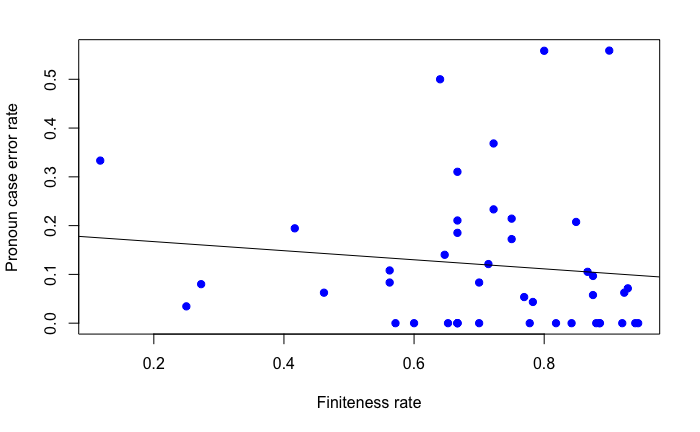
\includegraphics[scale = 0.5]{graph/Rispo1.png}
    \vspace{-1.5em}
    \caption{Pronoun case error rate by finiteness rate in CHILDES data }
    \label{fig:780}
\end{figure}
\FloatBarrier

\FloatBarrier
\begin{figure}[!h]
    \centering
    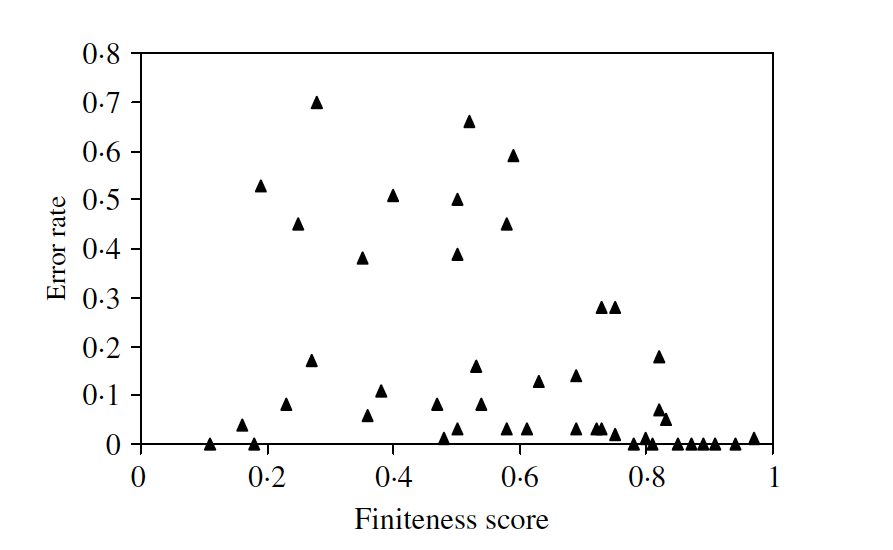
\includegraphics[scale = 0.4]{graph/Rispo2.png}
    \vspace{-1em}
    \caption{Pronoun case error rate by finiteness rate in \cite{rispoli2005}}
    \label{fig:781}
\end{figure}
\FloatBarrier

In conclusion, there is no significant correlation found between the pronoun case error rate and the finiteness rate in the CHILDES data. The regression analysis also demonstrates that the pronoun case error rate can not be predicted by verbal finiteness, age or mlu. \cite{rispoli2005}'s results were not replicated in CHILDES data.


\subsection{Conclusion}
This section reviewed the syntactic explanation for non-nominative subject errors, which claims that the use of the non-finite verbs leads to the non-nominative subject error in children's speech. It predicts that the presence of the finite verb will block the non-nominative subjects, therefore sentences like `*Her goes to the school' should almost never occur. Generally, it is difficult to test this prediction since non-nominative pronouns are rarely used as the subject. Therefore, it's difficult to judge if it is rare for the non-nominative subjects to precede a finite verb since the non-nominative subjects are uncommon. 

One way to test if the finite verb lowers the likelihood of the non-nominative pronoun is to compare the conditional probability of non-nominative subjects given finite verb P(Non-nominative|Finite) to the probability of non-nominative subjects P(Non-nominative). If P(Non-nominative|Finite) is smaller than P(Non-nominative), then it means that the presence of the finite verb actually prevents the use of non-nominative subjects. The meta-analysis shows that in general P(Non-nominative) is significantly larger than P(Non-nominative|Finite). However, depending on the child and the pronoun, P(Non-nominative) is often no different from P(Non-nominative|Finite). This result indicates that the finite verb doesn't guarantee that the subject pronoun will always get the nominative case, which is against the prediction of the syntactic explanation. In addition, the pronoun case error rate and the finiteness rate is not correlated, indicating that when children use more finite verbs, they don't necessarily make fewer pronoun case errors. The regression analysis also showed that the pronoun case error can not be predicted by finiteness rate. 

In conclusion, there is not enough evidence to support hypothesis that pronoun case errors stem from children's use of non-finite verbs. The finite verb does not always block the use of non-nominative subjects, and there is also no correlation between the finiteness rate and the pronoun case error rate. 